% document class using the Springer publishing company's document class
\documentclass[envcountsame,envcountchap]{svmono}

% packages to include additional functionality
\usepackage{makeidx}         % allows index generation
\usepackage{graphicx}        % standard LaTeX graphics tool
                     	       % when including figure files
\usepackage{multicol}        % used for the two-column index
\usepackage[bottom]{footmisc}% places footnotes at page bottom
\usepackage{wrapfig} % for wrapping images with text
\usepackage{color} % for coloring links
\usepackage{fancyvrb}
\usepackage{amssymb} %for symbols like arrows
\usepackage{listings} %for inserting code 
\usepackage{pdfpages} %to insert pdf
\usepackage[hyphens]{url}
\usepackage{hyperref} %to insert url
\usepackage{nameref}
\begin{document}
\author{Srividya Majeti}
\title{Assignment 6}

\subtitle{CS 532:  Introduction to Web Science\\Dr. Michael Nelson\\Spring 2016}

% note that this special command is part of the document class
% and, in addition to creating the title page, also inserts the 
% current date on the page
\maketitle

\frontmatter

\tableofcontents

\mainmatter

% include other tex files so we don't have one huge document to scroll through
\chapter{Question 1}
\label{intro}

\textbf{Demonstrate that you know how to use ``curl'' well enough to correctly POST data to a form. Show that the HTML response that is returned is ``correct''.  That is, the server should take the arguments you POSTed and build a response accordingly.  Save the HTML response to a file and then view that file in a browser and take a screen shot.}\\

To POST data to a form using cURL, I did the following:
\begin{itemize}
\item I created a form using PHP with name as an input element and a submit button.

\item When we open this PHP form in the browser and type any name, it displays a response saying ``Welcome followed by the text''.

\item By using the following cURL command we can POST data to the form which is received by the server and generates a response with the same message that we see on the browser. By using -o followed by parameter, I am outputting the HTML response to a file.
\end{itemize}
\begin{verbatim}
 curl -d name=Srividya ``www.cs.odu.edu/~smajeti/postForm.php'' 
 -o output.html
\end{verbatim}


\newpage

\lstinputlisting[language=PHP,caption=``PHP script'',frame=single,breaklines=true,captionpos=b,numbers=left,showspaces=false,showstringspaces=false,basicstyle=\footnotesize]{src/postForm.php}

\begin{figure}[h!]
\begin{center}


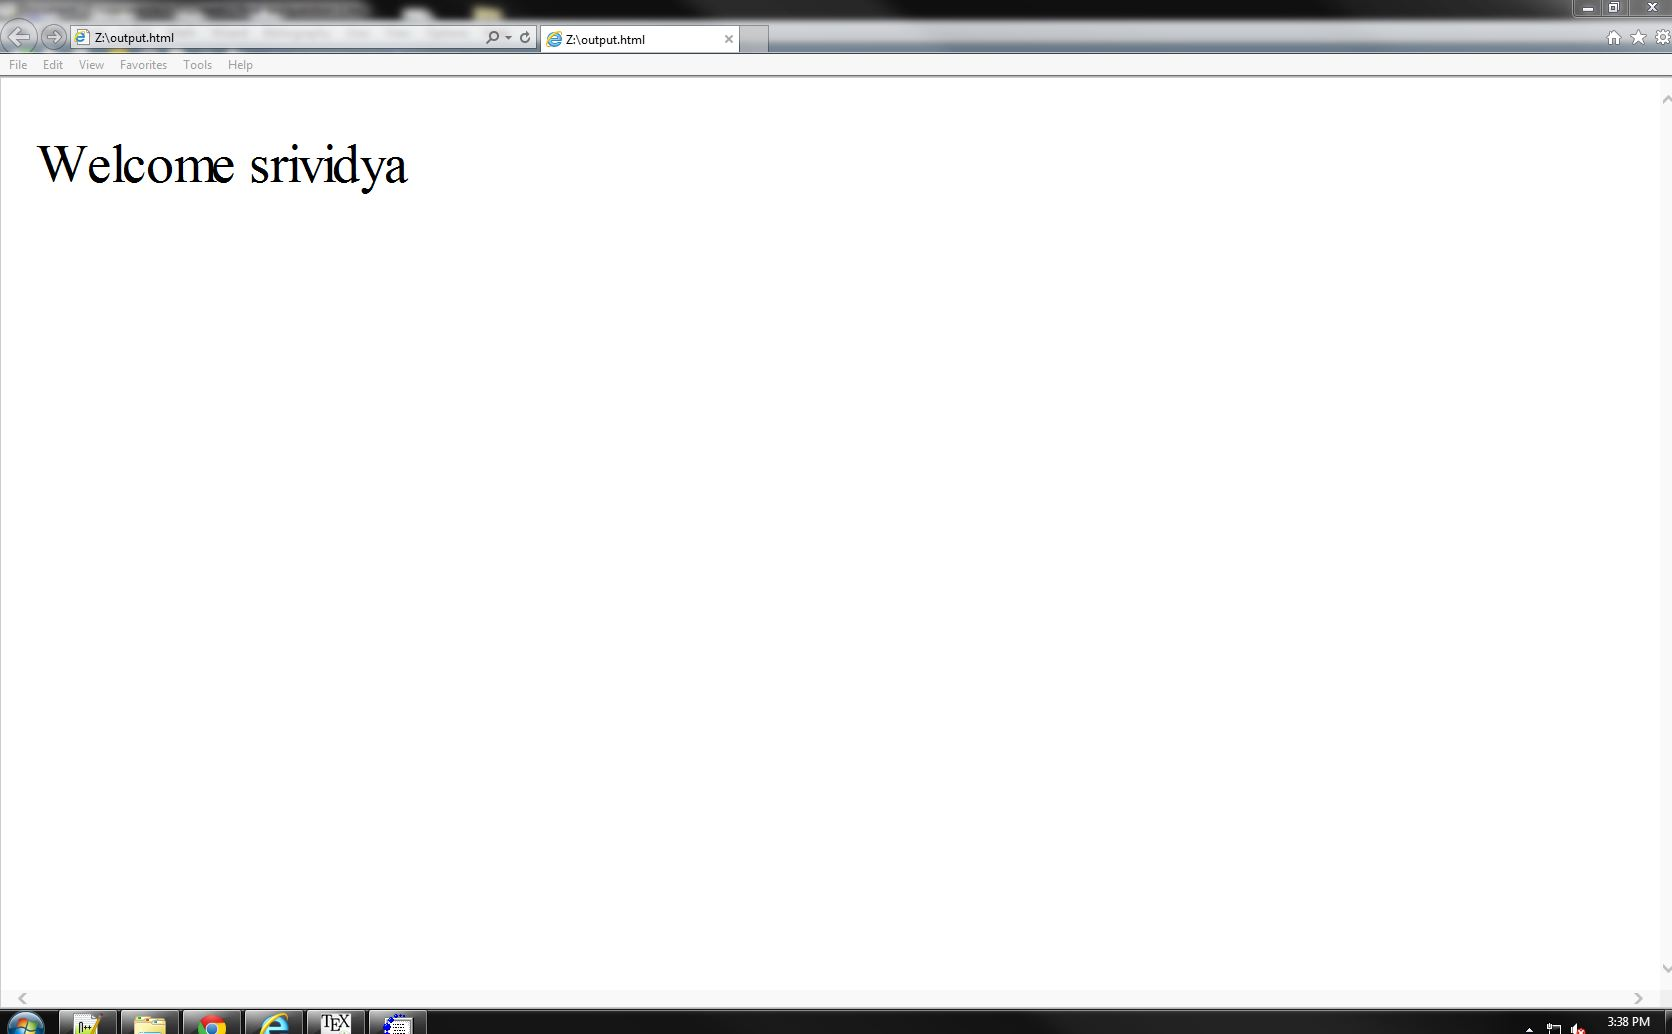
\includegraphics[scale=0.30, keepaspectratio=true]{figures/q1screenshot.JPG}
\caption{HTML response saved into a file and viewed in browser.}
\label{mcpon_navy_mil}
\end{center}
\end{figure}

\chapter{Question 2}
\label{avoiding-uri-aliases} 

\textbf {Determine if the friendship paradox holds for your Twitter account. Since Twitter is a directed graph, use ``followers'' as value you measure
(i.e., ``do your followers have more followers than you?'').\\
Generate the same graph as in question 1, and calcuate the same  mean, standard deviation, and median values.\\
For the Twitter 1.1 API to help gather this data, see:}\\
{\url{https://dev.twitter.com/docs/api/1.1/get/followers/list}}\\
\textbf{If you do not have followers on Twitter (or don't have more than 50), then use my twitter account ``phonedude\textunderscore mln''.}

Following are the steps that I have taken to solve this problem:
\begin{itemize}
\item I did not have more than 50 followers, so I randomly picked a user with the screen name `ohttic' from your followers list. He has 258 Followers and is following 1,923 people.
\item Twitter provides an API to get the list of followers. This API returns an object of followers with the profile information. `Tweepy' library is a wrapper around Twitter that makes it easier to retrieve Twitter data. I used this library to get the followers data.
\item I iterated through the list of users and retrieved the `screen\textunderscore name', `followers\textunderscore count' and `friends\textunderscore count'. I stored this information in a JSON structure and saved it into a file `userFollowerdata' . This code is listed in Listing \ref{lst:q2code1}.
\item Furthermore, I extracted the followers count from the JSON and stored it in a file `followersCount'. This code is listed in Listing \ref{lst:q2code2}
\item I calculated the mean, median and standard deviation for the followers count. This code is listed in Listing \ref{lst:q2code3}. The mean, median and standard deviation are given in Table \ref{Table:q2table1}

\begin{table}

\caption{Mean, Median and Standard Deviation of number of followers of followers}
\label{Table:q2table1}
\begin{center}
\begin{tabular}{| c | c |}
\hline
Key & Value \\ \hline

Mean & 54474.2 \\ \hline
Median & 5477.0 \\ \hline
Standard Deviation & 120893.613437 \\ \hline

\hline

\end{tabular}
\end{center}
\end{table}

\newpage
\item Figure \ref{fig:q2fig2} illustrates the ranking of `ohttic' in terms of followers count in comparison with his followers.
\begin{figure}[h!]
\begin{center}
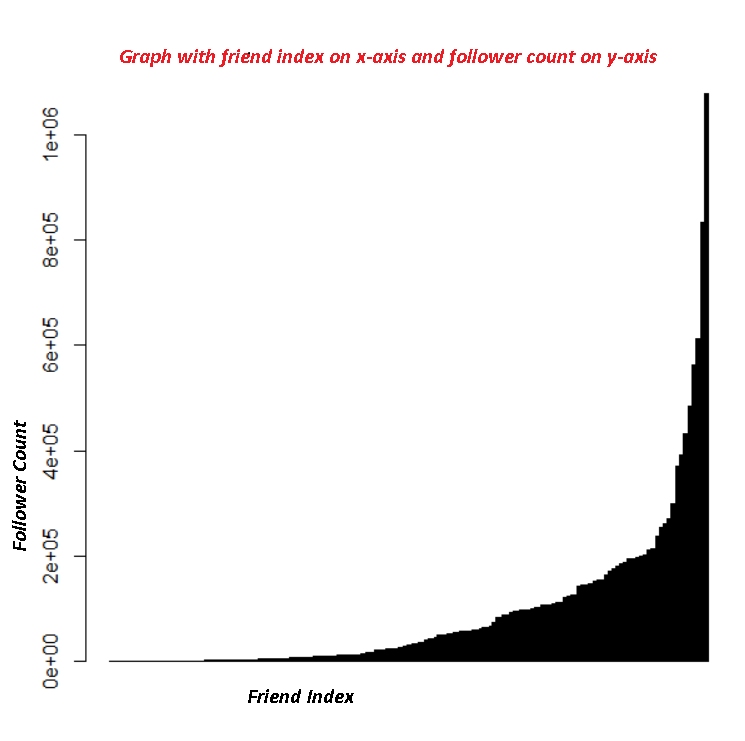
\includegraphics[scale=0.55, keepaspectratio=true]{figures/followerWithoutLog.PNG}
\caption{Graph with number of followers on y-axis and followers on x-axis }
\label{fig:q2fig2}
\end{center}
\end{figure}

\begin{figure}[h!]
\begin{center}
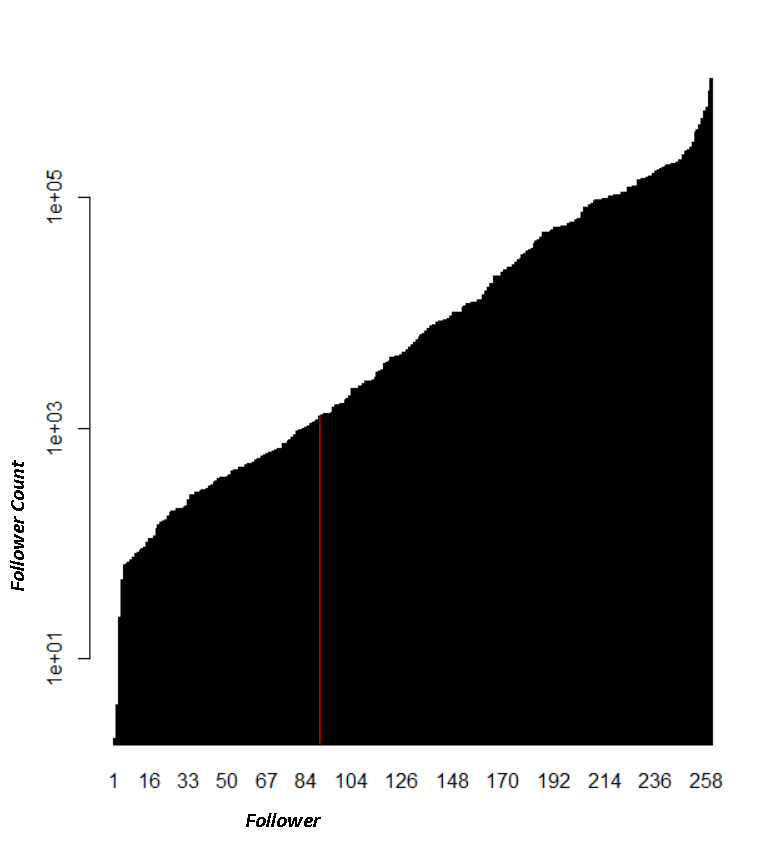
\includegraphics[scale=0.55, keepaspectratio=true]{figures/finalFollower.PNG}
\caption{Graph with number of followers on y-axis in log scale and followers on x-axis }
\label{fig:q2fig3}
\end{center}
\end{figure}
\newpage
\item From the calculated median value `5477.0' and number of followers `ohttic' have `258' we can say that he have less number of followers than his followers.

\end{itemize}

\newpage
\textbf{Code Listing}
\lstinputlisting[language=Python,caption=Python code for retrieving friends data and storing screenName followersCount and friendsCount in a JSON structure ,frame=single,label=lst:q2code1,breaklines=true,captionpos=b,numbers=left,showspaces=false,showstringspaces=false,basicstyle=\footnotesize]{src/getFollowerAndFriendsData.py}

\newpage
\textbf{Code Listing}
\lstinputlisting[language=Python,caption=Python code for extracting followers count from JSON structure,frame=single,label=lst:q2code2,breaklines=true,captionpos=b,numbers=left,showspaces=false,showstringspaces=false,basicstyle=\footnotesize]{src/extractFollowers.py}

\textbf{Code Listing}
\lstinputlisting[language=Python,caption=Python code for calculating mean median and standard deviation,frame=single,label=lst:q2code3,breaklines=true,captionpos=b,numbers=left,showspaces=false,showstringspaces=false,basicstyle=\footnotesize]{src/getMeanMedianStandardDeviation2.py}
\chapter{Question 3}
\label{available-representation}

\textbf{Re-download the 1000 TimeMaps from A2, Q2.  Create a graph where the x-axis represents the 1000 TimeMaps.  If a TimeMap has ``shrunk'', it will have a negative value below the x-axis corresponding to the size difference between the two TimeMaps.  If it has stayed the same, it will have a ``0'' value.  If it has grown, the value will be  positive and correspond to the increase in size between the two TimeMaps.\\\\
As always, upload all the TimeMap data.  If the A2 github has the  original TimeMaps, then you can just point to where they are in  the report. }\\\\

Following are the steps I have taken to solve the problem:
\begin{itemize}
\item I repeated the same process that I did in Assignment 2 for getting the mementos data.
\item With the help of ODU Memento Aggregator, I downloaded TimeMaps for all the URIs that are extracted in Assignment 2 question 1 using the following curl command:\\
{\url {curl -i --silent http://mementoproxy.cs.odu.edu/aggr/timemap/link/1/<uri>}}\\
These URIs are located at \url{https://github.com/majetisiri/cs532-s16/blob/master/a2/uri.json}.
\item  I stored the output produced by the cURL command into a file `PagesList'. 
\item I processed the data from the above file to create a JSON with the original URI, memento URI , datetime and memento count. The memento count for each URI is derived by counting the URIs with rel=``memento''. This is outlined in Listing \ref{lst:q3code1}.
\item Using `getTimeMaps.py' I wrote the memento count for all the 1000 URIs for Assignment 2 and Assignment 10 in 2 different files `allMementosA2' and `allMementosA10' respectively.This code is listed in Listing \ref{lst:q3code2}.
\item I calculated the difference between TimeMaps for Assignment 10 and Assignment 2 and stored the output in `differenceTimemaps'. This code is illustrated in Listing \ref{lst:q3code3}
\item The output graph where the x-axis represents the 1000 TimeMaps is illustrated in Figure \ref{fig:q3fig1}. 
\begin{figure}[h!]
\begin{center}
\hspace*{-3cm} 
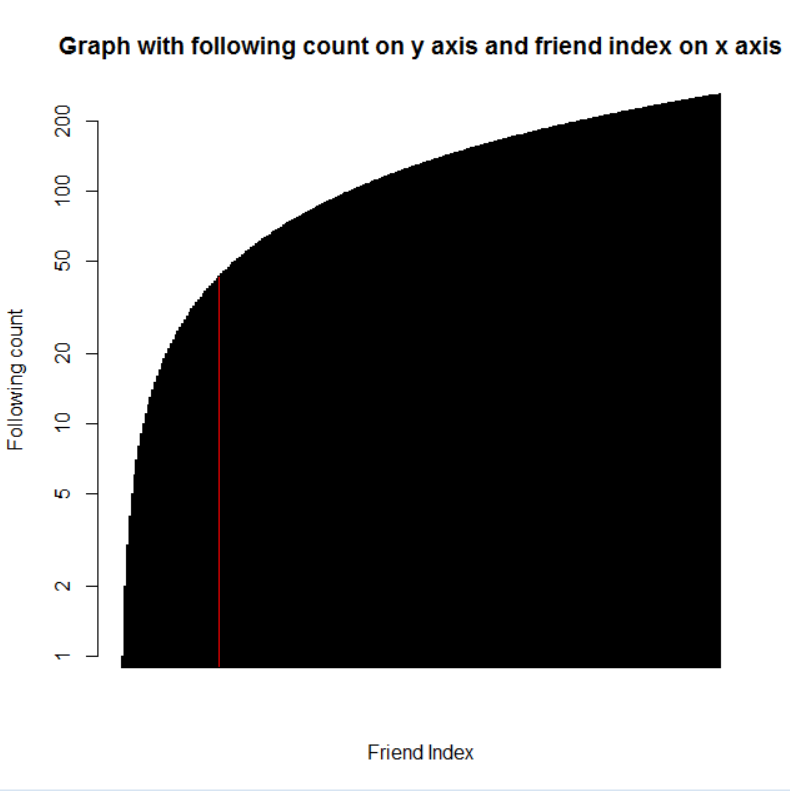
\includegraphics[scale=0.55, keepaspectratio=true]{figures/1.PNG}
\caption{Output graph with time maps on x axis}
\label{fig:q3fig1}
\end{center}
\end{figure}
\item From this graph we can conclude that most of the TimeMaps are `grown' as the value is positive. But we can see few TimeMaps are `shrunk' which have negative values.
\end{itemize}

\newpage
\textbf{Code Listing}
\sloppy
\lstinputlisting[language=Python,caption= Python code for getting mementos data.,frame=single,breaklines=true,label=lst:q3code1, tabsize=2, captionpos=b,numbers=left,showspaces=false,showstringspaces=false,basicstyle=\footnotesize]{src/getMementosData.py}


\textbf{Code Listing}
\sloppy
\lstinputlisting[language=Python,caption=python code for getting time maps from mementos data.,frame=single,breaklines=true,label=lst:q3code2, tabsize=2, captionpos=b,numbers=left,showspaces=false,showstringspaces=false,basicstyle=\footnotesize]{src/getTimeMaps.py}

\newpage
\textbf{Code Listing}
\sloppy
\lstinputlisting[language=Python,caption=python code for getting difference in time maps for mementos in Assignment 2 and Assignment 10.,frame=single,breaklines=true,label=lst:q3code3, tabsize=2, captionpos=b,numbers=left,showspaces=false,showstringspaces=false,basicstyle=\footnotesize]{src/getDifference.py}

\chapter{Question 4}
\label{available-representation}

\textbf{Use MDS to create a JPEG of the blogs similar to slide 29. How many iterations were required?}\\\\

Following are the steps I have taken to solve the problem:

\begin{itemize}
\item I imported the `clusters.py' mentioned in `question 2' and used the code described in `presentation slide 29' to create a JPEG of the most similar blogs using MDS. This code is in Listing \ref{lst:q4code1} 
\newpage
\item The output JPEG file is illustrated in \ref{fig:q4fig1}. 
\begin{figure}[h!]
\begin{center}
\hspace*{-3cm} 
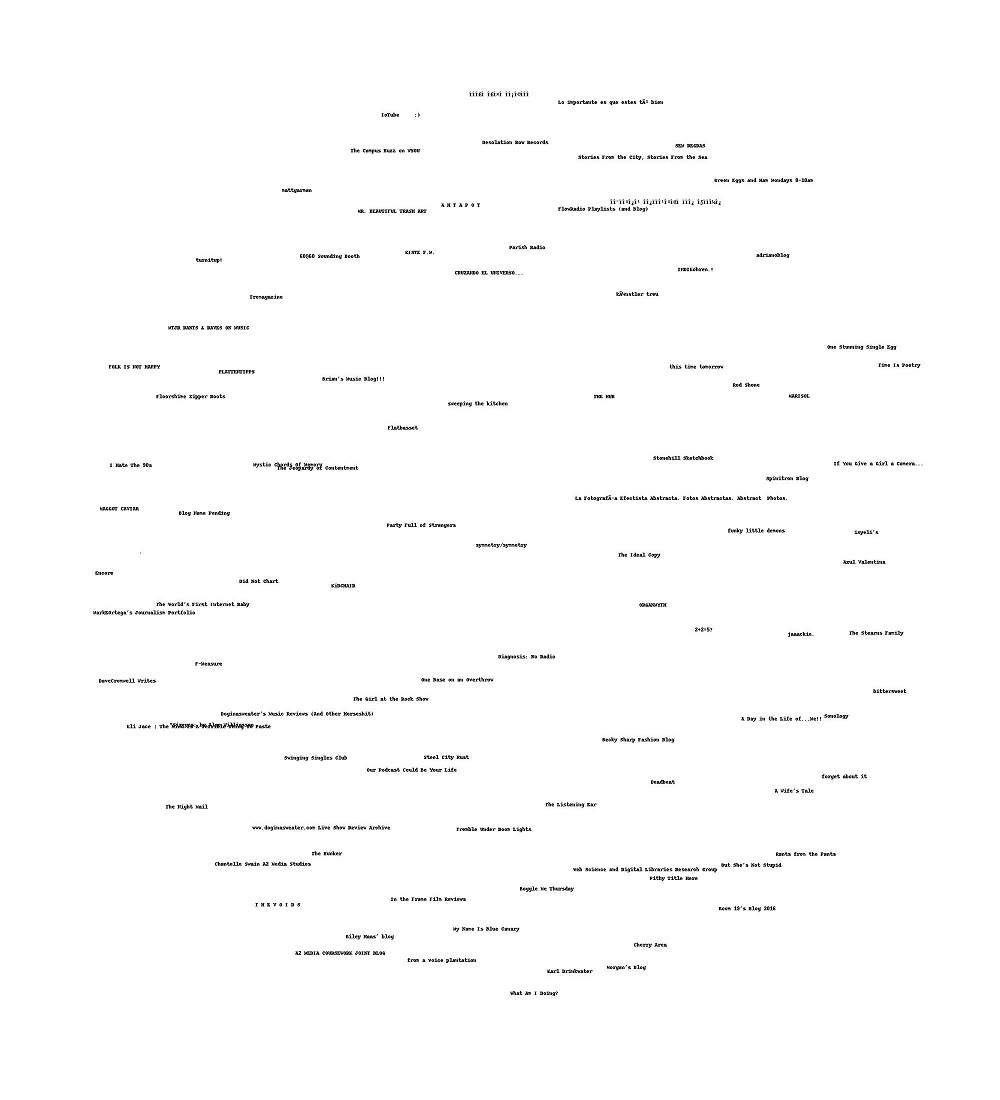
\includegraphics[scale=0.55, keepaspectratio=true]{figures/blogs2d.jpg}
\caption{JPEG of blogs using MDS}
\label{fig:q4fig1}
\end{center}
\end{figure}
\item To get the number of iterations I have written a print statement in function `scaledown(data,distance=pearson,rate=0.01)' of `clusters.py'. `304'  iterations were required for creating the JPEG using MDS. The file `numberOfIterations.txt' has `total error' and `iteration count'.
\item The python code `clusters.py' that I downloaded from the PCI book is illustrated in Listing \ref{lst:q4code2}
\end{itemize}


\textbf{Code Listing}
\sloppy
\lstinputlisting[language=Python,caption=Python code for creating MDS,frame=single,breaklines=true,label=lst:q4code1, tabsize=2, captionpos=b,numbers=left,showspaces=false,showstringspaces=false,basicstyle=\footnotesize]{src/createMDS.py}


\textbf{Code Listing}
\sloppy
\lstinputlisting[language=Python,caption=Python code `clusters.py' from PCI ,frame=single,breaklines=true,label=lst:q4code2, tabsize=2, captionpos=b,numbers=left,showspaces=false,showstringspaces=false,basicstyle=\footnotesize]{src/clusters.py}
\chapter{Extra-Credit Question-3}
\label{intro}

\textbf{Rank the 1,682 movies according to the 1997/1998 MovieLense data.  Now rank the same 1,682 movies according to todays (March 2016) IMDB data (break ties based on number of users, for example: 7.2 with 10,000 raters $>$ 7.2 with 9,000 raters).\\
Draw a graph, where each dot is a film (i.e., 1,682 dots).  The x-axis is the MovieLense ranking and the y-axis is today's IMDB
ranking. \\
What is Pearon's r for the two lists (along w/ the p-value)?  Assuming the two user bases are interchangable (which might not be a good
assumption), what does this say about the attitudes about the films after nearly 20 years?}\\


Following are the steps I have taken to solve the problem:

\begin{itemize}
\item I ranked all the movies based on MovieLense. The python code for this is illustrated in \ref{lst:q5code1}
\item Futhermore I ranked all the movies based on todays IMDB data. The python code for this is illustrated in \ref{lst:q5code2}
\item For IMDB data I got the ranking out of 10.0, I normalized the ranking to 5.0.
\newpage
\item The output file for MovieLense with rating and movie names are in Figure \ref{fig:q5fig1}.
\begin{figure}[h!]
\begin{center}
\hspace*{-3cm} 
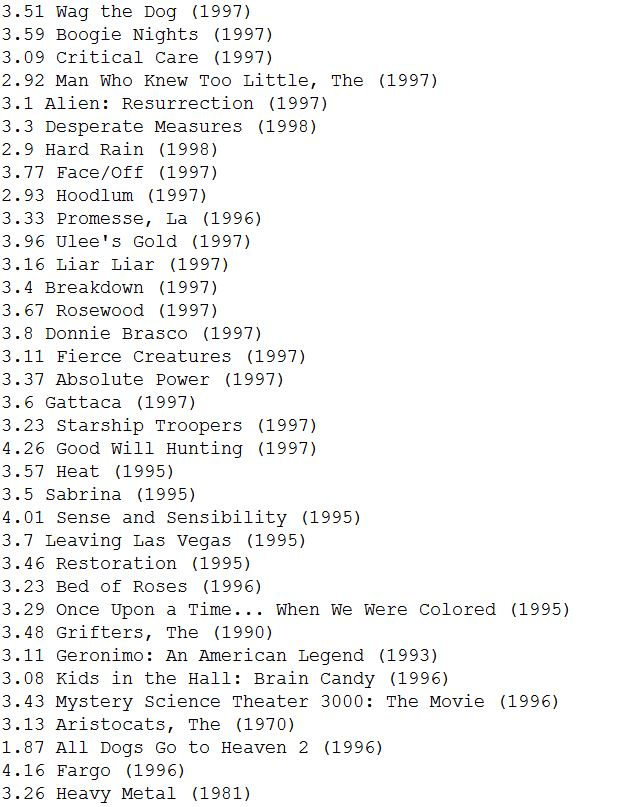
\includegraphics[scale=0.55, keepaspectratio=true]{figures/2.JPG}
\caption{MovieLense rating}
\label{fig:q5fig1}
\end{center}
\end{figure}
\newpage
\item The output file for IMDB with rating and movie names are in Figure \ref{fig:q5fig2}
\begin{figure}[h!]
\begin{center}
\hspace*{-3cm} 
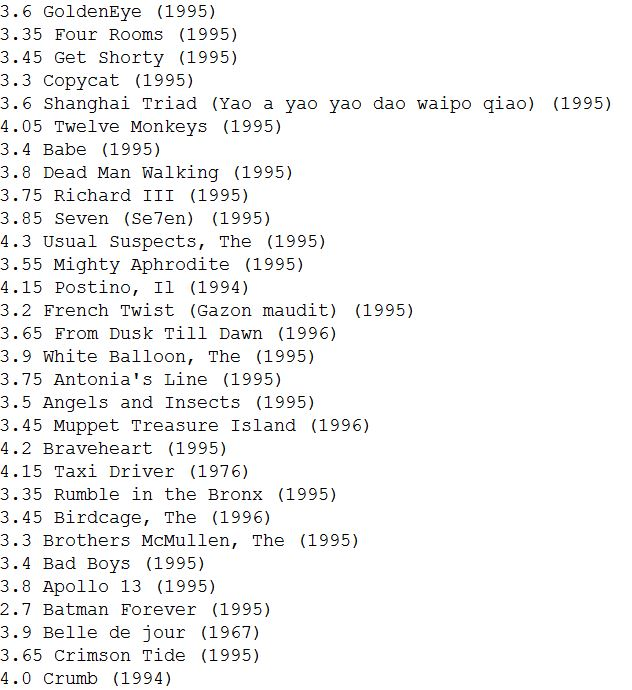
\includegraphics[scale=0.55, keepaspectratio=true]{figures/3.JPG}
\caption{IMDB rating}
\label{fig:q5fig2}
\end{center}
\end{figure}
\end{itemize}

\newpage
\textbf{Code Listing}
\sloppy
\lstinputlisting[language=Python,caption=Python code for ranking movies based on MovieLense data.,frame=single,breaklines=true,label=lst:q5code1, tabsize=2, captionpos=b,numbers=left,showspaces=false,showstringspaces=false,basicstyle=\footnotesize]{src/rankBasedOmovieLense.py}

\newpage
\textbf{Code Listing}
\sloppy
\lstinputlisting[language=Python,caption=Python code for ranking movies based on IMDB data.,frame=single,breaklines=true,label=lst:q5code2, tabsize=2, captionpos=b,numbers=left,showspaces=false,showstringspaces=false,basicstyle=\footnotesize]{src/getIMDB.py}

\backmatter
\bibliographystyle{ieeetr} 		
\nocite{*}  					
\small  					

\bibliography{Master}

\end{document}